\begin{frame}
\frametitle{Vigencias futuras e inversión pública (\% PIB)}

\begin{figure}
    \centering
    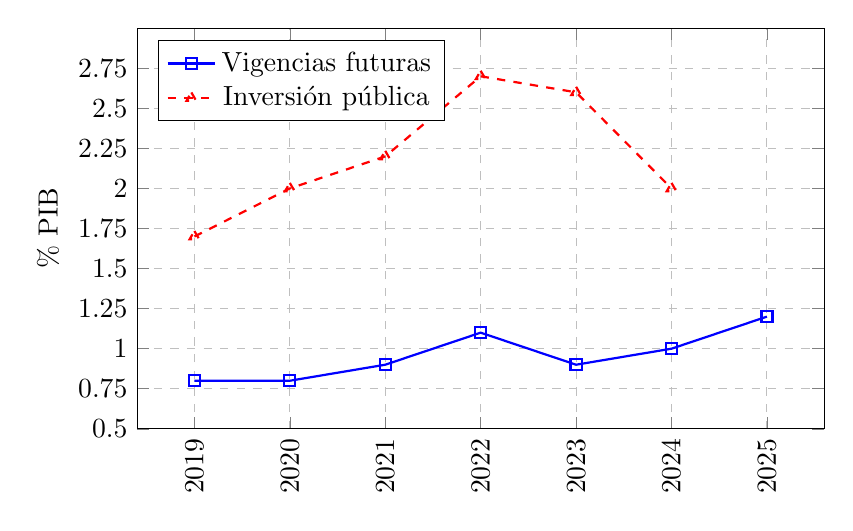
\begin{tikzpicture}
        \begin{axis}[
            width=0.85\textwidth,
            height=0.55\textwidth,
            grid=major,
 %           xlabel={Año},
            ylabel={\% PIB},
            ymin=0.5, ymax=3.0,
            xtick={2019,2020,2021,2022,2023,2024,2025},
            xticklabel style={rotate=90,anchor=east,/pgf/number format/.cd,1000 sep={},fixed,precision=0},
            scaled x ticks=false,
            ytick={0.50,0.75,1.00,1.25,1.50,1.75,2.00,2.25,2.50,2.75},
            legend pos=north west,
            ymajorgrids=true,
            xmajorgrids=true,
            grid style=dashed,
        ]

        % Vigencias futuras
        \addplot[
            color=blue,
            mark=square,
            thick
        ]
        coordinates {
            (2019,0.8)
            (2020,0.8)
            (2021,0.9)
            (2022,1.1)
            (2023,0.9)
            (2024,1.0)
            (2025,1.2)
        };

        % Inversión pública
        \addplot[
            color=red,
            mark=triangle,
            dashed,
            thick
        ]
        coordinates {
            (2019,1.7)
            (2020,2.0)
            (2021,2.2)
            (2022,2.7)
            (2023,2.6)
            (2024,2.0)
        };

        \legend{Vigencias futuras, Inversión pública}

        \end{axis}
    \end{tikzpicture}

    \vspace{0.3cm}
%    \par\footnotesize{\textit{Fuente: Elaboración propia con base en Marcos Fiscales de Mediano Plazo 2018--2024 y Balance del GNC, Ministerio de Hacienda.}}
\end{figure}

\end{frame}
